\chapter{Introduction}


% am Ende der alten Intro...
% hier fehlt mir eine klare Beschreibung der Problemstellung...du bist sehr generisch und sagst, dass es vor und nachteile hat, benennst diese aber nicht
% Was auch fehlt ist dein Lösungsvorschlag bzw. deine Idee, wie man die Problemstellung bearbeiten kann (was du in dieser Arbeit vorhast)




% 1. Absatz: Beschreibe uns das Forschungsfeld in dem du dich befindest (DevOps / GitOps)

%\noindent
Increasingly more organizations are adopting 
a DevOps culture to develop new applications and services at high velocity. 
After all, a culture that encourages shared responsibility, transparency and rapid feedback, 
helps to narrow the gaps between teams and thus accelerate the development process.
In order to
reduce friction between engineering teams who are involved in the software development lifecycle (SDLC),
a new practice called GitOps has emerged.
It allows developers who are already familiar with the revision control system Git,
to easily deploy their applications to target environments in a self-service model.
System administrators and operators can also manage IT infrastructure
purely by interfacing with declarative state definitions stored in Git.
%GitOps is a set of principles for operating and managing software systems.
%These principles are derived from modern software operations, but also have their roots 
%in existing and widely adopted best practices. 
\bigskip

%\noindent
%The primary four principles,
%which serve as principles for the desired state of a
%system managed by GitOps are the following \autocite{gitopsPrinciplesv100}:
%
%\begin{itemize}
%	\item \textbf{Declarative} \\
%		A system managed by GitOps must have its desired state expressed declaratively.
%	\item \textbf{Versioned and Immutable} \\
%		Desired state is stored in a way that enforces immutability, versioning and retains a complete version history.
%	\item \textbf{Pulled Automatically} \\
%		Software agents automatically pull the desired state declarations from the source.
%	\item \textbf{Continuously Reconciled} \\
%		Software agents continuously observe actual system state and attempt to apply the desired state.
%\end{itemize}
%
%% TODO: ensure list does not lap over multiple pages in PDF export
%
%\noindent
%These principles are defined in OpenGitOps version 1.0.0,
%which is a Cloud Native Computing Foundation (CNCF) sandbox project
%in the App Delivery TAG 
%under the GitOps Working Group.
%The overall goal of OpenGitOps is to establish a clear vendor-neutral,
%principle-driven meaning of GitOps,
%which shall provide a foundation for interoperability between tools, conformance and certification through enduring programs, documents and code
%\autocite{opengitopsDocuments}.
%This thesis aims at adhering to the definitions in OpenGitOps
%for the term GitOps, its principles and the glossary around it.
%However, the research is not limited to the definitions in OpenGitOps,
%and might even suggest changes.




% 2. Absatz: Beschreib uns das Problem bzw. die Challenge in diesem Forschungsfeld (Was ist die Problemstellung, die es zu bearbeiten gilt)

% TODO: why is it important to solve the problem?

\noindent
GitOps as a practice for releasing software has many advantages,
but like other solutions, GitOps also has some shortcomings.
One of the unresolved problems is
the process of promoting releases between multiple deployment environments (illustrated in Figure \ref{fig:releasePromotionProcess}).

\begin{figure}[h]
	\centering
	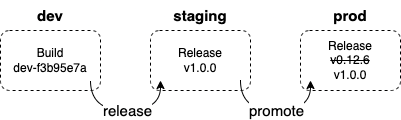
\includegraphics[width=.55\linewidth]{figures/release-promotion.drawio.png}
	\caption{release promotion process.
		%		(\citeauthor{ref}, \citeyear{ref}).
	}
	\label{fig:releasePromotionProcess}	
\end{figure}

\noindent
Current GitOps tools do not provide an integrated solution for this process,
nor do they provide any sort of abstraction for defining environments.
Users currently need to rely on separation of duties
on a file and folder level within the Git repository,
for modeling different environments.
Promotions are often achieved via hard-coded file copy operations,
which is done by the CI/CD system.
In addition, for each configuration or templating tool which is used
(e. g. kustomize, helm, jsonnet, etc.),
the modeling of different environments, as well as the
process of promotion, is unique.
This makes the process of promotion rather difficult.
Clear guidelines and best practices,
as well as tools which implement them,
are missing in the GitOps ecosystem.
\bigskip

% 3. Absatz: Was schlägst du vor, wie man die Problemstellung bearbeiten könnte? Beschreibe uns deinen Lösugnsvorschlag dieser Arbeit, wie man das Problem bearbeiten könnte

\noindent
%
The given problem could be addressed by
providing standardised models 
for defining deployment environments and promotion processes.
%
An application programming interface (API) extension for Kubernetes
could provide custom resource definitions for these models.
%
This would allow users to define abstract representations of
their environments,
and how they want releases to be promoted between them.
%
Additional logic could be introduced into the promotion process,
like specifying a rule which ensures that new releases must first pass
certain environments or other objectives before being promoted to production.
%
The abstraction would also enable transparent replacement of the
configuration or templating tool,
while keeping the desired state definition intact.
%
Following the principles of GitOps,
a controller would ensure the continuous reconciliation
between the desired and the actual state of the resources.
\bigskip

% 4. Absatz: gib uns einen Ausblick (Paint the Big Picture) wie deine Lösung mit dem großen Ganzen zusammenhängt

\noindent
%
The proposed solution of the problem should
present a possible way of defining environments and promotion processes abstractly,
onto which future work could build upon.
%
Additionally the solution should
provide a protoype of a toolkit,
which could serve as an optional component
in addition to existing tooling within the CNCF.
%
Solving the problem of release promotion natively within the GitOps toolkit,
would make the adoption of GitOps more appealing,
especially for organisations, which have the need for many different environments.
%
As a result
this could generally accelerate the widespread use of GitOps
and thus enable more organisations to develop higher quality software.
%








%Previously, this process was usually handled by the CI/CD system,
%which would execute a pipeline, in which every environment
%is being deployed to consecutively
%in an imperative way.
%With GitOps, the state of the different environments
%is completely defined
%in a declarative way.
%The system state is continuously reconciled
%by the GitOps controller.
%What turns out to be tricky,
%is the process of promotion to other deployment environments.


%In recent years with DevOps and Continuous Delivery practices,
%the release promotion process through different environments is becoming ever more important.
%Containerization technologies allow for easy deployments to
%uniquely different environments.
%However it is important to model different environments in
%a homogeneous way,
%in order to simplify the full automation of the software delivery process.


%\noindent
%In order to help with full automation of the 
%release and promotion process of new software releases,
%this gap needs to be filled.
%Not only larger organizations need a high level of automation.
%Smaller organizations also
%greatly benefit from automation, in order
%to deliver high quality software.
%\bigskip


%\noindent
%GitOps can be viewed as an evolution of Infrastructure as Code (IaC) that uses Git as a version control system for infrastructure configurations.
%GitOps lowers the cost of building self-service IT systems and enables self-service operations that were previously unjustifiable
%\autocite{limoncelli_gitopsPathToMoreSelfService}.
%It improves the ability to operate systems securely by
%allowing unprivileged users to make major changes,
%without granting these users direct access to the target system.
%Through so-called pull requests, ordinary users can submit a request
%of their proposed changes.
%These pull requests can then be reviewed and accepted by more privileged users.
%If necessary, adjustments can be suggested or incorporated by the reviewers themselves.
%\bigskip
%
%\noindent
%Security can be improved by adding automated tests.
%These tests can include
%Linting (validation of syntax),
%enforcing style guides,
%running end-to-end and unit tests,
%or
%enforcing security policies.
%Security reviews and audits become easier 
%because every change is tracked.
%Every change or commit is permanently recorded in the Git history
%\autocite{limoncelli_gitopsPathToMoreSelfService}.
%\bigskip





